\documentclass{tietreport}

% Import images
\usepackage{graphicx}

% Bibliography configuration
\usepackage[
  date=year,
  style=alphabetic,
  backend=biber,
  sorting=nty,
  maxnames=5,
  minnames=3,
  maxalphanames=4,
  minalphanames=3,
  backref=true,
  doi=false,
  isbn=false,
  url=false,
  eprint=false
]{biblatex}
\addbibresource{references.bib}

% Start chapters on the next page, not the next right-hand page, so no
% blank pages are inserted (the class itself stays unchanged).
\makeatletter
\@openrightfalse
\makeatother

%% ==================================================
%% CUSTOMIZE THESE FIELDS FOR YOUR PROJECT
%% ==================================================

% Course/Lab header
\TitlePageHeader{%
  UCS503 - Software Engineering%
}

% Main project title
\ProjectTitle{%
  Hostel Room Swapping Service%
}

% Subtitle or project description
\ProjectSubTitle{%
  Multi-Party Room Exchange Chains that Nobody Can See Alone%
}

% Student information (up to 4 students)
\author{%
  \texttt{1024030673} Aabhas Khandelwal \\
  \texttt{1024031097} Aakash Chawla \\
  \texttt{1024030674} Joy Soni%
}

% Group number, degree, year, program
\TitlePageSubText{%
  Group: \texttt{3C51} BE Third Year, CSE%
}

% Faculty advisor/guide name
\AdvisorName{%
  Dr. Raghav B. Venkataramaiyer%
}

% Evaluation period and department info
\TitlePageFooterText{{%
    \large End-Semester Evaluation \\[0.2cm]
    \bfseries Computer Science and Engineering
    Department%
  } \\[0.15cm]
  Thapar Institute of Engineering and Technology,
  Patiala%
}

%% ==================================================

\begin{document}

% Generate title page
\maketitle

% Table of contents (auto-generated from chapters)
\tableofcontents

% ===== CHAPTER 1: INTRODUCTION =====

\chapter{Introduction}

\section{Background and Context}

Hostel rooms at Thapar Institute are allotted once a semester, and the
allotment is fixed once it is made. Some students end up on the wrong
floor, in the wrong room type or away from their friends, and the only
remedy is informal: a post in a group chat, a few replies, rarely a
swap.

A direct swap rarely works, because it needs two students who each
want exactly what the other has. A rotation of three or more usually
does work: A takes B's room, B takes C's, and C takes A's, and everyone
gains. No student can see such a rotation from their own conversation,
because finding it needs every student's room and every student's
preferences at once.

The Hostel Room Swapping Service holds that information centrally. Its
key observation is that a swap round is a \emph{closed pool}: the only
rooms in play are the ones the participants already hold. Any solution
is therefore a permutation of students over beds, every permutation
splits uniquely into disjoint cycles, and those cycles are the swap
chains. The service computes them, offers each student the chains that
help them, and moves rooms only when every member of a chain agrees.

\subsection{Problem Statement}

Let $S$ be the $n$ students of a round and $B$ their $n$ beds, with
current allocation $\pi_0 : S \to B$, a bijection. Each student $s$ has
a feasible set $H_s \subseteq B$ (beds meeting all of their hard
preferences) and a score $u_s : B \to [0,1]$ (the share of their soft
preference weight a bed's room meets).

Find bijections $\pi$ with $\pi(s) \in H_s$ among the $K$ best by
$\sum_s u_s(\pi(s))$. Each cycle $C$ of $\pi \circ \pi_0^{-1}$ with
$2 \le |C| \le L$ is offered if and only if it is a Pareto improvement:
$u_s(\pi(s)) \ge u_s(\pi_0(s))$ for every $s \in C$, and
$u_s(\pi(s)) > u_s(\pi_0(s))$ for at least one $s \in C$. Each student
is shown at most three such cycles, and a cycle executes if and only if
every member approves within $T$. The live service uses $K = 50$,
$L = 8$ and $T = 3$ days.

The scope is one round for one hostel. The service must also survive
the realities of approval: a member may refuse, a member may never
answer, two chains may claim the same student, and the record of who
held which room must never be rewritten.

\section{Project Objectives}

\begin{enumerate}
  \item \textbf{Objective 1:} Offer only chains that leave nobody worse
    off. Measured as the number of students worse off after a round;
    target zero on every evaluated cohort.
  \item \textbf{Objective 2:} Offer chains short enough to be agreed.
    Target: no offered chain longer than a cap chosen by measurement,
    and a shorter longest chain than the single optimal assignment
    gives.
  \item \textbf{Objective 3:} Reach many students. Target: on
    300-student cohorts, at least half of the students offered an
    executable chain at the chosen cap.
  \item \textbf{Objective 4:} Never let one student block the others.
    Target: a refusal frees the whole chain at once; silence expires
    after three days; one live chain per student, enforced by the
    database and tested on PostgreSQL.
  \item \textbf{Objective 5:} Run fast enough for a warden to press one
    button. Target: a 100-student round in under ten seconds.
  \item \textbf{Objective 6:} Deliver a deployed web service with
    student and warden interfaces, an automated test suite in
    continuous integration, and documentation, by the end of the
    semester (August to November 2026).
\end{enumerate}

Each objective is specific and measurable, achievable with the team of
three, relevant to the problem above, and bound to the semester. All
six are evaluated in Chapter~\ref{ch:results}.

% ===== CHAPTER 2: METHODOLOGY & DESIGN =====

\chapter{Methodology and Design}

The service was built iteratively and incrementally
\cite{sommerville2016se}: each iteration delivered a working system
that was run, measured and improved. The work was tracked in Git, with a
\texttt{development} branch for integration and \texttt{main} for
releases.

\section{System Architecture}

\subsection{High-Level Design}

The service is a layered Python application behind a single-page web
interface. The layers have strict rules about what they may depend on:

\begin{itemize}
  \item The \textbf{domain engine} (\texttt{hostelswap/domain}) holds all
    of the matching mathematics and the proposal state machine. It
    imports no web framework and no database driver, so every part of
    it is tested with no infrastructure.
  \item The \textbf{data-access layer} (\texttt{db.py}) is the only
    module that contains SQL.
  \item The \textbf{workflow layer} (\texttt{rounds.py}) wires the two
    together and enforces the round rules. It contains no SQL and no
    matching logic.
  \item The \textbf{API layer} (\texttt{api.py}, \texttt{auth.py})
    authenticates requests, checks roles and serves the compiled React
    interface, so one process serves the whole application.
\end{itemize}

\paragraph{Bed slots.} A student's preferences are properties of a room,
but the assignment must be one-to-one, so every room is split into bed
slots, one per bed. The problem stays a permutation (as many slots as
participants) while shared rooms and roommate requests remain possible.

\paragraph{Data.} PostgreSQL holds 15 tables: students and sessions;
hostels, rooms and bed slots; the declared room types; the allocation
history; rounds and enrolments; preference sets; roommate requests;
stored chain options; and proposals with one row per chain member.
Three rules are enforced by the database itself: the allocation history
is append-only (triggers reject \texttt{UPDATE} and \texttt{DELETE});
a student has one active preference set per round; and a student sits
in at most one unsettled chain (a partial unique index).

\paragraph{Round lifecycle.} \texttt{draft} $\rightarrow$ \texttt{open}
$\rightarrow$ \texttt{locked} $\rightarrow$ \texttt{running}
$\rightarrow$ \texttt{completed}, or \texttt{cancelled} by a warden from
draft, open or completed. Locking closes registration and runs the
engine in one request, so priorities cannot change after the engine has
read them.

\paragraph{Proposal lifecycle.} One proposal is one chain. It stays
\texttt{proposed} while collecting replies; the first rejection makes it
\texttt{rejected} and frees every member; the last approval makes it
\texttt{approved}, and it is executed at once, appending one allocation
row per member; after three days without every approval it becomes
\texttt{expired}; a warden may make it \texttt{cancelled}. Chains from
one assignment are disjoint cycles, so a drop-out in one chain cannot
affect any other.

\paragraph{Alternatives considered.} Gale--Shapley stable matching
\cite{gale1962college} needs two-sided preferences, but rooms do not
rank students. Top Trading Cycles \cite{shapley1974cores} fits the
exchange shape but needs strict ranked lists, while our preferences are
weighted across several attributes.

\subsection{Technical Stack}

\begin{itemize}
  \item \textbf{Framework/Language:} Python 3.10--3.12 with FastAPI for
    the backend; TypeScript with React, built with Vite, for the
    interface.
  \item \textbf{Database:} PostgreSQL, hosted on Supabase, with the
    schema managed as numbered migrations (\texttt{db/migrate.py}).
  \item \textbf{Tools:} Git and GitHub, GitHub Actions for continuous
    integration and the documentation site, pytest, MkDocs, nginx on the
    deployment server.
  \item \textbf{Libraries:} SciPy (\texttt{linear\_sum\_assignment}) and
    NumPy for the matching engine, psycopg~3 with a connection pool,
    Uvicorn.
\end{itemize}

\section{Implementation Details}

\subsection{Module 1: Core Functionality}

The core functionality is the matching engine, a pipeline of pure
functions in \texttt{hostelswap/domain}.

\paragraph{Scoring.} A preference names a criterion (room, hostel,
floor, side, washroom, room type or roommate), a value, a weight and
whether it is hard. A room's score is the share of the student's soft
weight it meets; an unmet hard preference makes it infeasible instead.
The score keeps the lists of met and unmet preferences.

\paragraph{Cost matrix and the Hungarian algorithm.} Rows are students
and columns are bed slots; each cell is the negated score, or $\infty$
when infeasible. A tie-break of $10^{-9}$ on every slot but the
student's own keeps the solver from moving students between beds of the
same room for no gain. The matrix is solved with SciPy's
\texttt{linear\_sum\_assignment} \cite{virtanen2020scipy}, a
shortest-augmenting-path form of the Hungarian method
\cite{kuhn1955hungarian,munkres1957}. It assigns one student per phase,
and each phase finds an augmenting path while updating dual potentials
over the matrix in $O(n^2)$, so a solve costs $O(n^3)$. For a dense
matrix of real costs, no asymptotically faster exact method is used in
practice.

\paragraph{Murty's algorithm.} The single best assignment is often not
the useful one: it may demote a student, or need one very long chain.
Murty's algorithm \cite{murty1968ranking} enumerates the next best
assignments: for each edge of an assignment in turn it forbids that
edge, requires the edges before it, and solves again. The sub-problems
are disjoint and cover every other assignment, so nothing repeats and
nothing is missed. Each result creates up to $n$ sub-problems, each a
full solve, so $K$ results cost $O(K n^4)$ in the worst case.

\paragraph{Cycles and the Pareto filter.} Each assignment is split into
its cycles of length two or more. A cycle is kept only if nobody in it
is worse off and at least one member is better off. The check runs
after the solve, because the solver maximises the total, which can
legitimately demote one student to help several.

\paragraph{Options per student and the chain cap.} An early version
picked one plan for the whole hostel, which left most students with
nothing. The engine now collects every Pareto-improving chain from all
$K$ assignments, drops chains longer than the cap $L$, and keeps each
student's own three best. Chains shown to different students may
overlap on purpose: whoever offers first takes the rooms, and the
database stops a second chain from claiming the same student.

\subsection{Module 2: Secondary Features}

\paragraph{Round workflow.} \texttt{rounds.py} drives a round:
opening, enrolling and setting priorities while it is open, then
locking and running the engine, whose chains are stored so that page
loads never repeat the computation. A member of a stored chain offers
it, creating a proposal with a three-day deadline. Before inserting it,
the workflow expires every overdue proposal, so a chain nobody
answered cannot block the new one; no scheduler is needed. A reply
first checks the deadline, and a late reply is refused. A warden can
withdraw a single chain, or cancel a round, which cancels all of its
open chains and frees their members in one transaction.

\paragraph{Persistence.} \texttt{db.py} uses psycopg~3 with a
connection pool, and loads a student's round view in one query. The
schema lives in numbered SQL files applied in order by
\texttt{db/migrate.py}; an applied file is never edited. Migration
\texttt{0002} added a \texttt{settled} flag to chain members, so that
members of executed, rejected, expired or cancelled chains are free
again.

\paragraph{Security.} Passwords are stored as salted PBKDF2-HMAC-SHA256
hashes with 200\,000 iterations and compared in constant time
\cite{nist2017sp80063b}. A session is an opaque random token stored on
the server and carried in an \texttt{httpOnly}, \texttt{SameSite=Lax}
cookie that is \texttt{Secure} in production; logout deletes it. Every
student and warden route checks the role and answers 401 or 403. In
production the service refuses to start without a database, so it can
never show its demonstration data to real students.

\paragraph{Web interface and deployment.} The React interface has a
login page, a student page (current room, enrolment, priorities,
roommate requests, up to three chains with each member's move and match
percentage, and offers with a countdown to their deadline) and a warden
page (room types, round controls with a chain cap, every chain's
replies, withdraw and cancel). Its build is committed and served by
FastAPI. The service is deployed at
\texttt{hostelswap.aakashchawla.space} behind nginx; the documentation
site holds a tutorial, an API reference for all 34 routes and the
weekly journals.

\begin{figure}[h]
\centering
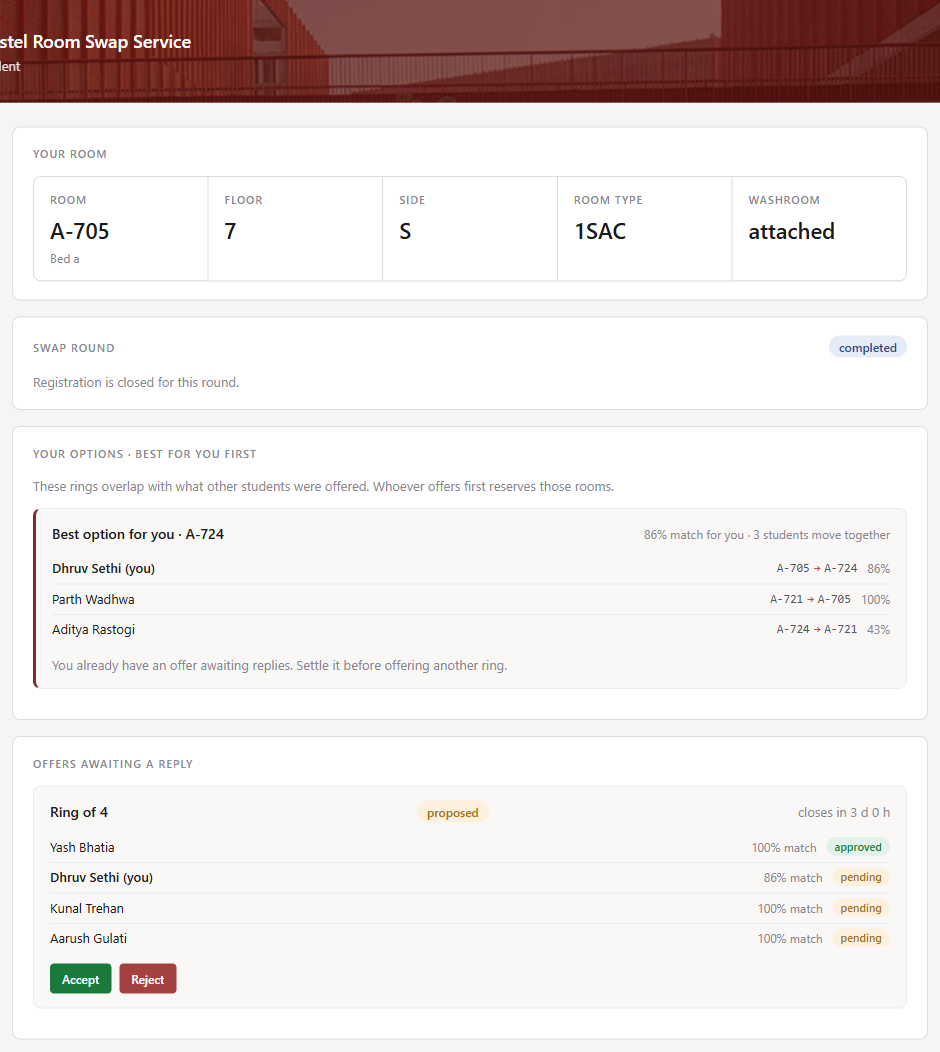
\includegraphics[width=0.72\textwidth]{figures/student.png}
\caption{Student page: current room, the student's best chains, and an
offer awaiting replies with its deadline}
\label{fig:student}
\end{figure}

\begin{figure}[h]
\centering
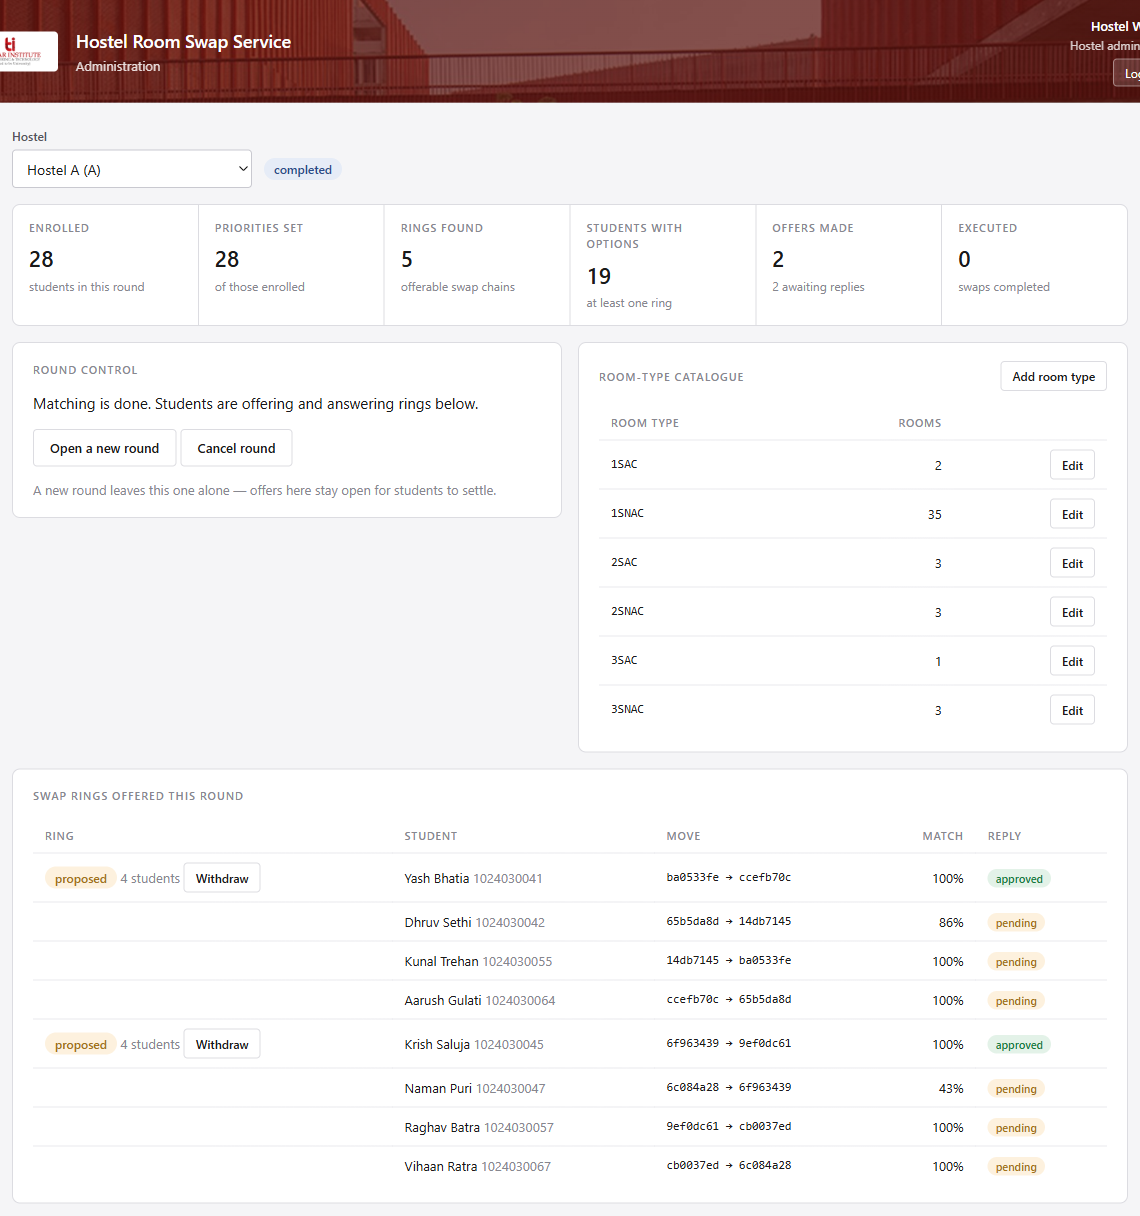
\includegraphics[width=0.85\textwidth]{figures/admin.png}
\caption{Warden page: round counts and controls, room types, and every
chain offered with each member's reply}
\label{fig:admin}
\end{figure}

% ===== CHAPTER 3: RESULTS & EVALUATION =====

\chapter{Results and Evaluation}
\label{ch:results}

\section{Testing Methodology}

\begin{itemize}
  \item \textbf{Unit Testing:} each domain module has its own tests:
    scoring (17), proposal states (15), ranking (15), generator (9),
    $k$-best (8), cycles, matrix and solver (7 each), pipeline and pool
    (6 each), feasibility (5). The $k$-best order is checked against a
    brute-force search over all 720 assignments of a 6-student pool.
  \item \textbf{Integration Testing:} nine golden scenarios run the full
    pipeline on hand-built hostels; the API is tested through FastAPI's
    test client (13); the database layer (14) and round workflow (10)
    are tested with stand-ins; and six tests run against a real
    PostgreSQL, three of which fail on the schema without migration
    \texttt{0002}. All 154 tests run in continuous integration on Python
    3.10, 3.11 and 3.12, with a throwaway PostgreSQL.
  \item \textbf{Performance Testing:} a golden test requires a
    100-student round to finish in under ten seconds; the benchmark
    script \texttt{benchmarks/chain\_cap.py} measures reach and run time
    on ten seeded 300-student cohorts.
  \item \textbf{User Testing:} no study with students has been run yet.
    The interfaces were checked by hand in a browser on a seeded round:
    offering, accepting, the deadline countdown, withdrawing a chain and
    cancelling a round.
\end{itemize}

No public benchmark exists for hostel swaps, so the cohorts are
synthetic and seeded, and the benchmark calls the same functions a live
round calls. Satisfaction is averaged over the whole cohort, not only
the students who move, so a two-person perfect swap cannot outrank a
rotation that lifts everyone; ``worse off'' is measured, not assumed.

\section{Performance Metrics}

\begin{table}[h]
\centering
\begin{tabular}{|l|r|r|}
  \hline
  \textbf{Metric} & \textbf{Target} &
  \textbf{Achieved} \\
  \hline
  Students worse off & $0$ & $0$ \\
  \hline
  Longest chain, 30 students & $< 28$ & $11$ \\
  \hline
  Offered a chain, 300 students & $\ge 50\%$ & $57.8\%$ \\
  \hline
  Run time, 100 students & $< 10$ s & passes \\
  \hline
  Automated tests in CI & all pass & $154$ of $154$ \\
  \hline
\end{tabular}
\caption{Performance Results Summary}
\label{tab:performance}
\end{table}

\paragraph{Frozen 30-student cohort.} One hostel, one student per room,
drawn once from a seeded generator and frozen. Each student's
priorities follow a ladder: a named room is worth more than its floor,
which is worth more than its side. The cohort is run through the
service's own \texttt{/api/demo} endpoint, which takes the best
assignment for the cohort among the $K$ explored.

\begin{table}[h]
\centering
\begin{tabular}{|l|r|r|r|}
  \hline
  \textbf{Metric} & $K=1$ & $K=50$ & $K=80$ \\
  \hline
  Satisfaction, before $\rightarrow$ after & 11\% $\rightarrow$ 77\% & 11\% $\rightarrow$ 77\% & 11\% $\rightarrow$ 77\% \\
  \hline
  100\% match (exact room) & 20 / 30 & 20 / 30 & 20 / 30 \\
  \hline
  Worse off & 0 & 0 & 0 \\
  \hline
  Longest chain needing approval & 28 & 11 & 11 \\
  \hline
  Run time & 0.03 s & 0.15 s & 0.16 s \\
  \hline
\end{tabular}
\caption{Frozen 30-student cohort}
\label{tab:demo}
\end{table}

\paragraph{Chain-cap benchmark.} Ten seeded cohorts of 300 students in
one hostel (seeds 1--10), $K = 200$, caps of 5, 8 and 10, reported as
mean $\pm$ population standard deviation. \emph{Offered}: students in at
least one chain within the cap among those they are shown.
\emph{Served}: students moved when chains are taken greedily, best mean
match first, without sharing a student. Mean satisfaction before any
swap is 34.4\%. The run is reproduced by \texttt{python
benchmarks/chain\_cap.py} in about eight minutes.

\begin{table}[h]
\centering
\begin{tabular}{|r|r|r|r|r|}
  \hline
  \textbf{Cap} & \textbf{Offered} & \textbf{Served} & \textbf{Satisfaction} & \textbf{Mean length} \\
  \hline
  5 & $28.0 \pm 7.2\%$ & $22.4 \pm 5.1\%$ & $47.2 \pm 3.2\%$ & 3.6 \\
  \hline
  8 & $57.8 \pm 8.8\%$ & $39.1 \pm 4.9\%$ & $57.0 \pm 3.3\%$ & 5.2 \\
  \hline
  10 & $71.9 \pm 9.0\%$ & $44.1 \pm 5.8\%$ & $60.1 \pm 3.8\%$ & 6.2 \\
  \hline
\end{tabular}
\caption{Chain-cap benchmark, 300 students, 10 seeds}
\label{tab:cap}
\end{table}

\paragraph{Scale.} The same script at 20, 40, 60, 80 and 100 students
shows why a large cohort is needed: at 20 students a chain of ten is
half the hostel, so the three caps land within five points of each
other (80--85\% offered); at 300 students cap 5 and cap 10 are 44 points
apart.

\section{Analysis}

\begin{itemize}
  \item \textbf{Did you meet your objectives?} Yes, on synthetic
    cohorts. Nobody was worse off in any cohort (Objective~1). Murty's
    alternatives cut the longest chain from 28 to 11 at the same 77\%
    satisfaction, and a cap of 8 was chosen by measurement
    (Objective~2). At cap 8, 57.8\% of students on 300-student cohorts
    are offered a chain (Objective~3). Refusal, expiry, one live chain
    per student and cancellation are enforced and tested on PostgreSQL
    (Objective~4). A 100-student round passes the ten-second test
    (Objective~5). The service is deployed with both interfaces, 154
    tests in CI and documentation (Objective~6).
  \item \textbf{Where did you exceed expectations?} The benchmark became
    fully reproducible: a committed script matches every reach figure
    of the original benchmark, including the spread, and all fifteen
    points of the scale study.
  \item \textbf{What challenges did you encounter?} Three stand out.
    First, proposals never expired: the domain defined the deadline but
    nothing called it, and the database index kept members of executed
    chains locked out. Second, the student page still showed members of
    expired chains as taken. Third, a change that ran Murty's search 13
    times faster, with every cost matching to $10^{-12}$, offered 3--10
    times fewer chains (seed 1, cap 8: 73.7\% $\rightarrow$ 14.7\% of
    students). These cohorts have very many assignments of exactly equal
    cost, and the two solvers broke those ties differently; $K = 200$
    sees only a small slice of the tied set.
  \item \textbf{How did you resolve them?} A deadline check on every
    reply, a sweep before every offer and migration \texttt{0002}; the
    results query now follows the same rule; and the faster solver was
    reverted, keeping only constant-time index lookups, which return
    identical assignments 1.1--1.5 times faster. Each fix has tests, and
    solver changes are now compared assignment by assignment, not by
    cost. Smaller challenges were the setup steps failing on a fresh
    clone and continuous integration not running on the team branch;
    both were fixed.
\end{itemize}

The main limitation is that every cohort is synthetic. Real preferences
may be more alike, for example everyone wanting the same floor, which
would lower every figure above. With cap 8, about 42\% of a
300-student cohort gets no offer, because a long cycle cannot be split
into shorter ones.

% ===== CHAPTER 4: CONCLUSION =====

\chapter{Conclusion}

\section{Summary of Work}

We built a service that turns a hostel's swap requests into one closed
assignment problem and reads the swap chains off its cycles. A pure
matching engine scores rooms, finds the best assignment with the
Hungarian algorithm and alternatives with Murty's algorithm, keeps only
chains in which nobody loses, and offers each student their own best
chains, capped at eight members. Around it sit a round workflow with an
approval state machine, deadlines and warden cancellation; a PostgreSQL
schema whose key rules are enforced by the database; a FastAPI backend
with session authentication; and a React interface for students and
wardens, deployed and documented. All six objectives were met on
synthetic cohorts.

\section{Key Findings}

\begin{itemize}
  \item \textbf{Finding 1:} The optimal assignment is not the useful
    one. Murty's alternatives cut the longest chain needing joint
    approval from 28 students to 11 with no loss in satisfaction.
  \item \textbf{Finding 2:} Chain length trades reach for agreement. On
    300 students, cap 8 offers 57.8\% of students a chain and cap 10
    71.9\%, but cap 10 serves only five points more at once.
  \item \textbf{Finding 3:} Reach depends on tie-breaking. Two exact
    solvers with identical costs offered up to ten times fewer chains
    apart, because the optimum is shared by very many assignments; an
    optimisation must be checked on the output that matters, not on an
    intermediate value.
\end{itemize}

\section{Future Work and Recommendations}

\begin{enumerate}
  \item A pilot round with real registrations in one hostel, to replace
    synthetic cohorts with real preferences.
  \item Break ties between equally good assignments deliberately, so
    that Murty's search visits more varied ones and reaches more
    students without a larger $K$.
  \item Warm-start each Murty sub-problem from its parent's dual
    potentials, needing one $O(n^2)$ augmenting path instead of a full
    solve, towards $O(K n^3)$, with reach measured again.
  \item Rate-limit login attempts, and notify students by email when a
    chain that includes them is offered, so fewer proposals expire.
  \item Run rounds for several hostels at once, and allow swaps between
    hostels where the institute permits them.
\end{enumerate}

\section{Final Remarks}

The central idea held: a closed pool makes swaps a matter of reading
cycles off one assignment. What we learned beyond it is that the
useful answer is the one a group of real students can agree on, which
is why the alternatives, the fairness filter, the cap and the deadline
matter as much as the solve itself, and that claims must be measured
again whenever the code changes. Every figure in this report can be
reproduced with the service's demo endpoint, the benchmark script and
the test suite.

% ===== BIBLIOGRAPHY =====

% Print bibliography with heading in TOC
\printbibliography[heading=bibintoc]

\end{document}
